%%==========================================================================%%
%% Author : Sa�udo Olmedo, Ignacio                                          %%
%% Author : S�nchez Barreiro, Pablo                                         %%
%% Version: 1.2, 23/04/2014                                                 %%
%%                                                                          %%
%% Memoria del Proyecto Fin de Carrera                                      %%
%% M2M/MetamodeloCassandra                                                  %%
%%==========================================================================%%

Previo paso a la definici�n de las reglas de transformaci�n entre modelos necesitamos definir un meta-modelo de origen y un meta-modelo de destino.Como hab�amos descrito en el capitulo anterior la base del proceso de transformaci�n entre modelos parte del meta-modelo. El meta-modelo de UML utilizado como origen en este proyecto es el que nos proporciona Epsilon, dicho meta-modelo sigue el est�ndar de UML 2.0. A parte del meta-modelo de UML nos hace falta un meta-modelo que defina el lenguaje de Cassandra. Dicho meta-modelo fue proporcionado por Pablo S�nchez Barreiro. Este meta-modelo se construyo por medio de la abstracci�n de las caracter�sticas de Cassandra. El meta-modelo sufri� algunos cambios respecto al inicial debido a exigencias y variantes que sufri� el proyecto. La Figura~\ref{back:fig:metamodeloCassandra} muestra un diagrama de clase UML que representa el modelo de datos. Este tipo de modelo es el origen del proceso de transformaciones entre modelos que queremos crear. A continuaci�n se detallan los aspectos mas importantes del meta-modelo de Cassandra.

\begin{figure}[!tb]
  \centering
  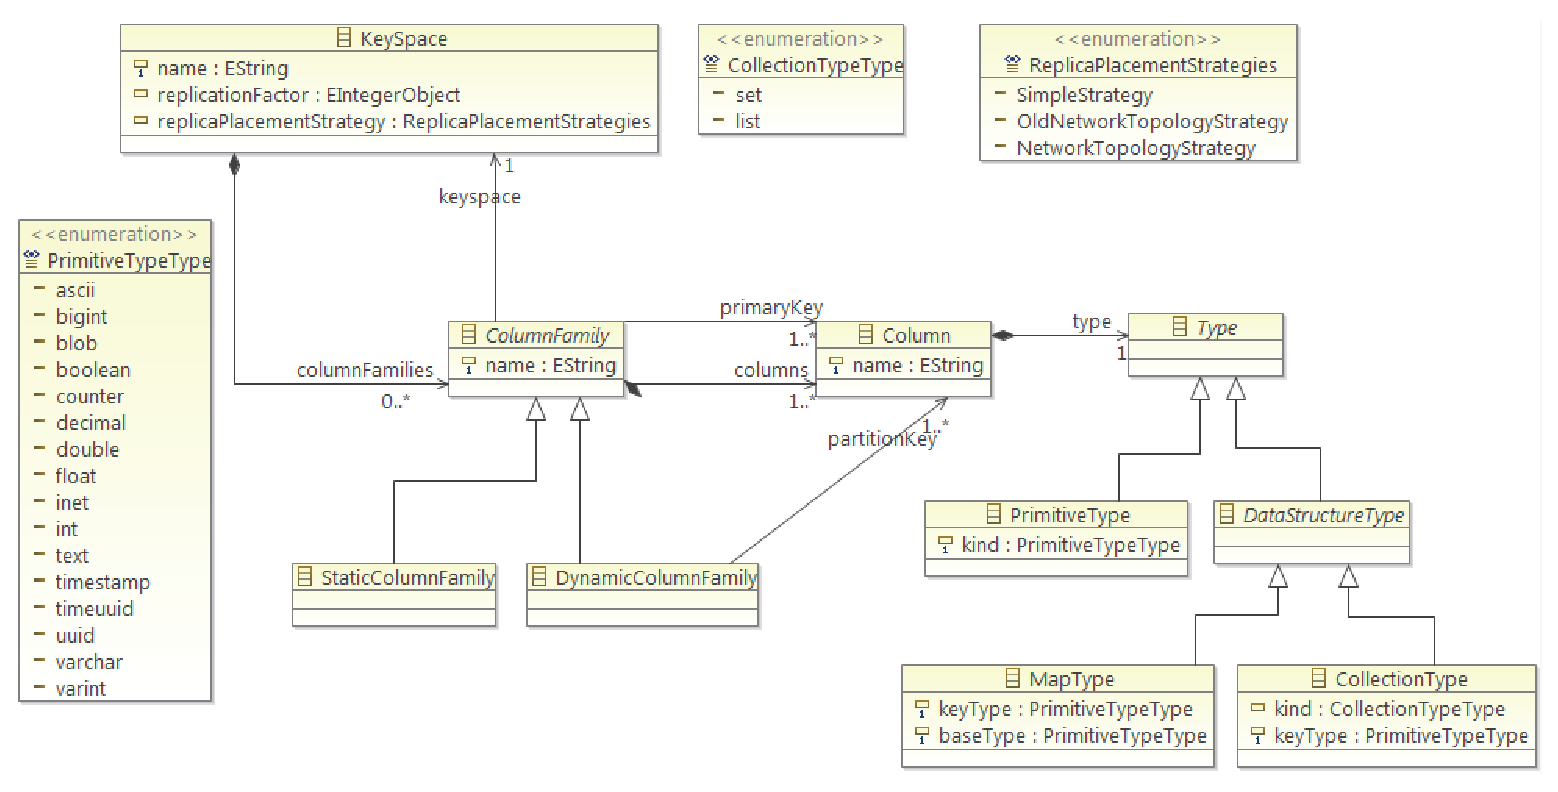
\includegraphics[width=.8\linewidth]{m2m/images/ecoreDiag.eps} \\
  \caption{Metamodelo Cassandra}
  \label{back:fig:metamodeloCassandra}
\end{figure}

De acuerdo con la estructura de Cassandra, el elemento ra�z de cualquier esquema orientado a columnas es el keyspace, el keyspace es el equivalente a la base de datos en el modelo relacional, la meta-clase keyspace cuenta con los meta-atributos: nombre utilizado para denominar el keyspace, [cassandra] replicationFactor que representa el n�mero de servidores de Cassandra de los que se debe guardar un registro u obtener una respuesta al recuperar alg�n registro y replicaPlacementStrategy es la estrategia de replicaci�n que se va a tomar, como estrategias tenemos tres tipos: %[http://www.datastax.com/docs/1.0/cluster_architecture/replication]:

\begin{enumerate}
\item SimpleStrategy: Es la estrategia de replicaci�n utilizada por defecto al crear un KeySpace utilizando Cassandra. Es utilizada para cl�steres de datacenters simples.
\item NetworkTopologyStrategy: Utilizada cuando se tiene (o se va a tener) el cl�ster desplegado a trav�s de m�ltiples data centers. Esta estrategia especifica cu�ntas r�plicas se desean en cada data center.
\item OldNetworkTopologyStrategy: Se utiliza para proporcionar retro compatibilidad con instalaciones Cassandra antiguas.
\end{enumerate}

A continuaci�n tenemos la meta-clase ColumnFamily equivalente a las tablas en el modelo relacional, dentro de esta meta-clase encontramos dos tipos: las StaticColumnFamily y las DynamicColumnFamily. Recordamos que las static column family son el equivalente a las tablas en el modelo relacional, sin embargo las dynamic column family son utilizadas para la recuperaci�n de datos eficiente, algo similar a las vistas del modelo relacional. %[http://www.datastax.com/docs/1.1/ddl/column_family#dynamic-column-families].

A la hora de definir las claves de las column families hay que tener en cuenta el orden, en CQL el orden de definici�n de las claves importa, en la primera columna se define la partition key, esta tiene la propiedad de que todas las filas que comparten la misma partition key se almacenan en el mismo nodo f�sico. %[http://www.datastax.com/docs/1.1/ddl/indexes].
Adem�s, la inserci�n, actualizaci�n o eliminaci�n de filas que comparten la partition key para una column family determinada se realizan de forma at�mica. Es posible tener una partition key compuesta, es decir, una partition key formada por varias columnas, en CQL esto se define utilizando par�ntesis para delimitar el conjunto de partici�n. En la siguiente columna se define la clustering key utilizada para la recuperaci�n de filas de manera eficiente.
Aunque en siguientes secciones esta informaci�n se amplia, el resumen de la definici�n de column families din�micas es la siguiente: PRIMARY KEY((partitioning key\_1, ... partitioning key\_n), clustering key\_1 ... clustering key\_n)


La siguiente meta-clase es Column, esta meta-clase contiene los valores que se almacenan en las Column Families, estas Columns tienen como meta-atributos un nombre y un tipo de dato.
Dentro de los tipos de datos que pueden darse en una columna encontramos dos tipos, PrimitiveType y DataStructureType, el primero define los tipos primitivos, por ejemplo entero, texto, uuid, etc..
DataStructureType define las colecciones. Estas pueden ser de dos tipos: MapType o bien CollectionType, ambas colecciones tienen un meta-atributo llamado KeyType para definir el tipo primitivo que utilizan. MapType cuenta con un meta-atributo llamado baseType de tipo primitivo que define el segundo tipo de dato del mapa. Dentro de CollectionType encontramos un meta-atributo llamado kind que define el tipo de colecci�n que vamos a utilizar, esta puede ser o bien tipo set o tipo list. M�s adelante se explica que caracter�sticas re�ne cada colecci�n y mapa y cuando se utilizan.
